\documentclass[a4paper, 12pt]{article}


\usepackage[french]{babel}
\usepackage[utf8]{inputenc}
\usepackage[T1]{fontenc}
\usepackage{lmodern}
\usepackage{listings}
\usepackage{graphicx}
\usepackage{amsmath}
\usepackage{amsfonts}
\usepackage{amssymb}
\usepackage{caption}
\usepackage{subcaption}
\usepackage[usenames,dvipsnames]{xcolor}


\setcounter{secnumdepth}{4}
% TAILLE DES PAGES (A4 serré)

\setlength{\parindent}{0pt}
\setlength{\parskip}{1ex}
\setlength{\textwidth}{17cm}
\setlength{\textheight}{24cm}
\setlength{\oddsidemargin}{-.7cm}
\setlength{\evensidemargin}{-.7cm}
\setlength{\topmargin}{-.5in}

% Commandes de mise en page
\newcommand{\fichier}[1]{\emph{#1}}
\newcommand{\nom}[1]{\emph{#1}}
\newcommand{\Fig}[1]{Fig \ref{#1} p. \pageref{#1}}
\newcommand{\itemi}{\item[$\bullet$]}

% Commandes de maths
\newcommand{\fonction}[3]{#1 : #2 \to #3}
\newcommand{\intr}[2]{\left[ #1 ; #2 \right]}
\newcommand{\intn}[2]{\left[\![ #1 ; #2 \right]\!]}
\newcommand{\intro}[2]{\left] #1 ; #2 \right[}
\newcommand{\intrsod}[2]{\left[ #1 ; #2 \right[}
\newcommand{\ps}[2]{\langle #1, #2 \rangle}
\newcommand{\mdelta}[1]{\boldsymbol{\delta_{#1}}}
%% \newcommand{\mdelta}[1]{\delta_{\textbf{#1}}}

\pagenumbering{arabic}
\graphicspath{{images/}}

\title{ASM-TP1 : Cancer de la prostate} 
\author{Pierre Petitbon \and Florian Privé \and Xinrui Xu}
\date{}

\begin{document}

\maketitle

\section{Analyse préliminaires des données}

\begin{enumerate}

\item On visualise sous R la matrice de corrélation entre lpsa et les 8 prédicteurs. 

\begin{center}
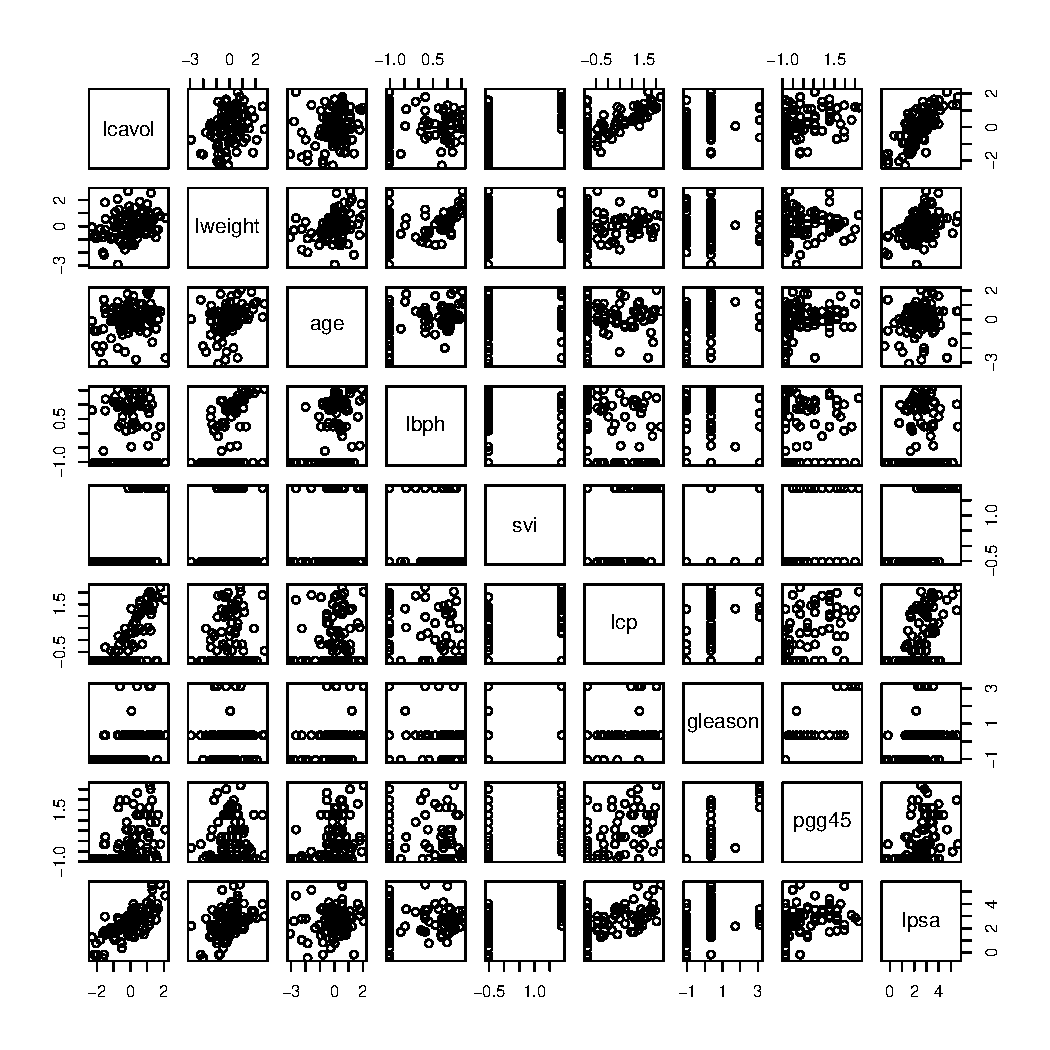
\includegraphics[scale=0.5]{Rplots.pdf}
\captionof{figure}{Rplots}
\label{fig1}
\end{center}

À partir du graphe précédent, on peut voir que certains facteurs sont corrélés ou pas avec lpsa. Pour cela, il suffit de regarder si le nuages de points forme plus ou moins une ellipse. 

\begin{tabular}{|p{0.5cm}|p{1.5cm}|p{1.5cm}|p{1.5cm}|p{1.5cm}|p{1.5cm}|p{1.5cm}|p{1.5cm}|p{1.5cm}|}
  \hline
       & lcavol & lweight & age & lbph & svi & lcp & gleason & pgg45 \\
  \hline
  lpsa & corrélé & non 

   corrélé & non 

    corrélé & non

     corrélé & corrélé & corrélé & non

      corrélé & non

       corrélé \\
  \hline 
\end{tabular}


\item 
À partir du graphe précédent, on peut aussi conjecturer s'il y a corrélation entre les prédicteurs.

\begin{tabular}{|p{1.4cm}|p{1.4cm}|p{1.4cm}|p{1.4cm}|p{1.4cm}|p{1.4cm}|p{1.4cm}|p{1.4cm}|p{1.4cm}|p{1.4cm}|}
  \hline
       & lcavol & lweight & age & lbph & svi & lcp & gleason & pgg45 \\
  \hline
  lcavol &  & non 

  corrélé & non 

   corrélé & corrélé & corrélé & corrélé & corrélé & corrélé \\
  \hline 
  lweight & non 

  corrélé & & non

  corrélé & non

  corrélé & non 

  corrélé & corrélé & corrélé & non

   corrélé \\
   \hline
   age & non 

   corrélé & non 

   corrélé &  & corrélé & corrélé & non 

   corrélé & corrélé & non 

   corrélé \\
   \hline
   lbph & corrélé & non 

   corrélé & corrélé & & corrélé & 
   non 

   corrélé & non 

   corrélé &
   non

   corrélé \\
   \hline
   svi & corrélé & non 

   corrélé & corrélé & corrélé & & corrélé & non 

   corrélé & corrélé \\
   \hline
   lcp & corrélé & corrélé & non 

   corrélé & non 

   corrélé & corrélé &  & corrélé & non

    corrélé \\
    \hline
    gleason & corrélé & corrélé & corrélé & non 

    corrélé & non 

    corrélé & corrélé & & corrélé \\
    \hline
    pgg45 & corrélé & non 

    corrélé & non 

    corrélé & non 

    corrélé & corrélé & non 

    corrélé & corrélé & \\
    \hline

\end{tabular}

\end{enumerate}



\section{Régression linéaire. Méthodes des moindres carrés.}

\begin{enumerate}
\item
La régression classique consiste à estimer les coefficients $\beta_{j}$ intervenant dans la relation suivante :

$ Y_{i} = \sum\limits_{j=1}^6 \beta_{j} x_{ij} + \beta_{0} + \sum\limits_{l=2}^4 \beta_{gleason, l} \mathds{1}_{x_{gleason, i}=l} + \epsilon_{i} $

où $Y$ représente lpsa et les $x_{j}$ représente les prédicteurs.  

D'après les résultats obtenus, les prédicteurs qui semblent influer le plus sur lpsa sont :
\begin{itemize}
\item lcavol (***) : on prend un risque très faible (p-valeur $=2.9x10^{-8}\%$) en disant que $\beta_{lcavol} \neq 0$.
\item lweight (**) : p-valeur $=0.25\%$.
\item svi (**) : p-valeur $=0.31\%$.
\item age (*) : p-valeur $=4.4\%$.
\end{itemize}




\end{enumerate}

\end{document}

% TODO : parler du scrum master
